%!TEX root = mb.tex



\section{Cryptographic Building Blocks}
\label{sec:buildingblocks}

In this section we present the building blocks \sys relies on.
Symmetric-key encryption (based on AES) is well known, and we do not discuss it here. Instead, we briefly discuss KeywordMatch (introduced by~\cite{blindbox}, to which we refer the reader for details) and more extensively discuss PrefixMatch, a new cryptographic scheme we designed for this setting.
When describing these schemes we refer to the encryptor as the gateway whose secret key is $k$ and to the entity computing on the encrypted data as the service provider (SP).


\subsection{KeywordMatch}\label{s:kwmatch}


KeywordMatch allows detecting if an encrypted keyword matches an encrypted data item by equality.
For example, given an encryption of the keyword ``malicious'', and a list of encrypted strings  [$\Enc$(``alice''), $\Enc$(``malicious''), $\Enc$(``alice'')], SP can  detect that the keyword matches the second string. 
For  this, we use a searchable encryption scheme~\cite{song:search, blindbox}.
Using this scheme, the gateway can encrypt a value $v$ into $\enc(v)$ and a rule $r$ into $\encr$ and SP can detect if there is a match between $v$ and $r$. 
 The security of searchable encryption is well studied~\cite{song:search, blindbox}: at a high level,  given a list of encrypted strings, and an encrypted keyword, SP does not learn anything about the encrypted strings, other than which strings match the keyword. 
 The encryption of the strings is {\em randomized}, so it does not leak whether two encrypted strings are equal to each other, unless, of course, they both match the encrypted keyword. 
  We use the technique from~\cite{blindbox} and hence do not elaborate on it.

%!TEX root = mb.tex

%\section{Building block: Range match}
%An important operation over an encrypted packet is to determine if an encrypted field in the packet falls in an encrypted range.
%We will use the firewall as an example. 
%Consider the following firewall rule:
%
%Constructing an encryption scheme that allows checking if an encrypted value is in an encrypted range, has been a challenge in the applied cryptography community. The reason is that ..
%
%\begin{itemize}
%\item preserve the order between Encryptd values
%\item candidate: OPE
%\item candidate: mOPE
%\item So none of the existing schemes are satisfactory. A new scheme \RM.
%\end{itemize}
%
%\RM applies to cases when we know an upper bound on the values encrypted with OPE and this is a small number of values (say, less than 10,000).
%
%The small number of values permits us to improve in two ways over mOPE [1]
%No more interaction. We store the tree in mOPE on the gateway (client) side, which means that the gateway can compute a new encryption by itself without help from service provider. The storage at the gateway will remain small.
%Rare updates to ciphertexts. We can space out the ciphertexts of the values encrypted sufficiently. 
%
%This also enjoys a stronger security than OPE! It leaks less than order.
%The reason is that, the server does not learn the order between the values in packets, and only whether they map between two values in the rules. 
%
%this one is new
%
%discuss 
%
%would be good to explain the challenge from the 
%
%\todo{a more interesting name to the scheme}
%
%prefix gets mapped into interval, at most a certain number
%
%talk about building certain data structures that all works the same
%
%firewall need not change 

\subsection{PrefixMatch} \label{sec:range}

\todo{what is the size of $\slen$, $\plen$, and $\ptlen$? we need to be consistent in all the examples}


Many middleboxes perform detection over {\it prefixes} or {\it ranges} of port numbers or IP addresses (i.e. packet classification). For example, a network administrator might wish to block access to all servers hosted by MIT, in which case the administrator would block access to the prefix 18.0.0.0/8, \ie{}, 18.0.0.0-18.255.255.255. PrefixMatch enables a middlebox to tell whether an IP address $v$ lies in between a range $[s_1, e_1)$, where $s_1$ = 18.0.0.0 and $e_1$ = 19.0.0.0; however, the middlebox does not learn the values of $v$, $s_1$, or $e_1$. Unlike KeywordMatch, PrefixMatch is a new scheme we designed specifically for our setting.

One might ask whether PrefixMatch is necessary, or one can instead employ KeywordMatch using the same expansion technique we used for some (but not all) regexps in \S\ref{sec:bbarch}. 
To detect whether an IP address is in a range, one could enumerate all IP addresses in that range and perform an equality check. However, the overhead of using this technique for common network ranges such as firewall rules is prohibitive.
For our own department network, doing so would convert our IPv6 and IPv4 firewall rule set of only 97 range-based rules to $2^{238}$ exact-match only rules; looking only at IPv4 rules would still lead to 38M exact-match rules.
Hence, to perform typical middlebox behaviors {\it in practice}, we require a PrefixMatch scheme which is more efficient.




\mypara{Functionality}
PrefixMatch encrypts a set of ranges or prefixes $P_1, \dots, P_n$ into a set of encrypted prefixes. For each $P_i$, there is one or more corresponding encrypted prefixes: $\ov{P}_{i,1} \dots, \ov{P}_{i, n_i}$.  Additionally, \pmatch{} encrypts a value $v$ into an encrypted value $\ov{v}$. These encryptions have the  property that, for all $i$,  
%
\[  v \in P_i  \Leftrightarrow \ov{v} \in \ov{P}_{i, 1} \cup \dots \cup \ov{P}_{i, n_i}. \]
%
In other words, the encryption preserves prefix matching.

For example, suppose that encrypting $P$ = 18.0.0.0/8 results in one encrypted prefix $\ov{P}$ = 2001:db8:85a3:0::::/64, encrypting $v_1$ = 18.0.0.2 results in  
 $\ov{v_1}$ = 2001:db8:85a3:0:0:8a2e:370:7334, and encrypting $v_2$ = 2:0:3:0:0:0:1:2 results in 
$\ov{v_2}$ = dc2:108:16:992:a53:43a:bb:c2. We can see that $\ov{v_1} \in \ov{P}$ and $\ov{v_2} \notin \ov{P}$. 

\todo{some of the below might have to move somewhere else}
Our goal in designing PrefixMatch was for it to be both efficient/fast {\em and} to provide strong security.



In terms of performance, both encryption (performed at the gateway) and detection (performed at the middlebox) should be practical for typical middlebox line rates.
Our PrefixMatch encrypts in $< 0.5\mu$s per value (we evaluate in \S\ref{sec:eval}).
Our design performs comparison between encrypted values and an encrypted rule (performed at the middlebox) using only on normal $\leq$/$\geq$ operators; hence it is compatible with existing classification algorithms such as tries, area-based quadtrees, FIS-trees, or hardware-based algorithms~\cite{packet_classif}.

For security, we require that the encryption scheme not leak $v$ to SP.
SP must not learn anything about $v$ other than which encrypted rule it matches to. 
In particular, even if both tuples $v_1$ and $v_2$ match the same rule, SP should not learn the order between them for each field of the tuple.
PrefixMatch also provides a level of security for the endpoints of the $j$-th range of rules:
 $s_{1j}$, $e_{1j}$, $\dots$, $s_{nj}$, $e_{nj}$. SP should not learn their values, and SP should not learn the order relation of the intervals. To the best of our knowledge, PrefixMatch is the only practical encryption scheme that achieves these security guarantees.

Although PrefixMatch has a similar functionality to order-preserving encryption such as BCLO~\cite{boldyreva:ope} or mOPE~\cite{popa:mope}, neither meets our security requirement (because they leak the ordering between encrypted values, not just whether they match a range) or provides the performance necessary for packet processing (as we show in \S\ref{sec:eval}).

\subsubsection{Scheme} 
\label{sec:rmscheme}

\begin{figure}[t]
  \centering
  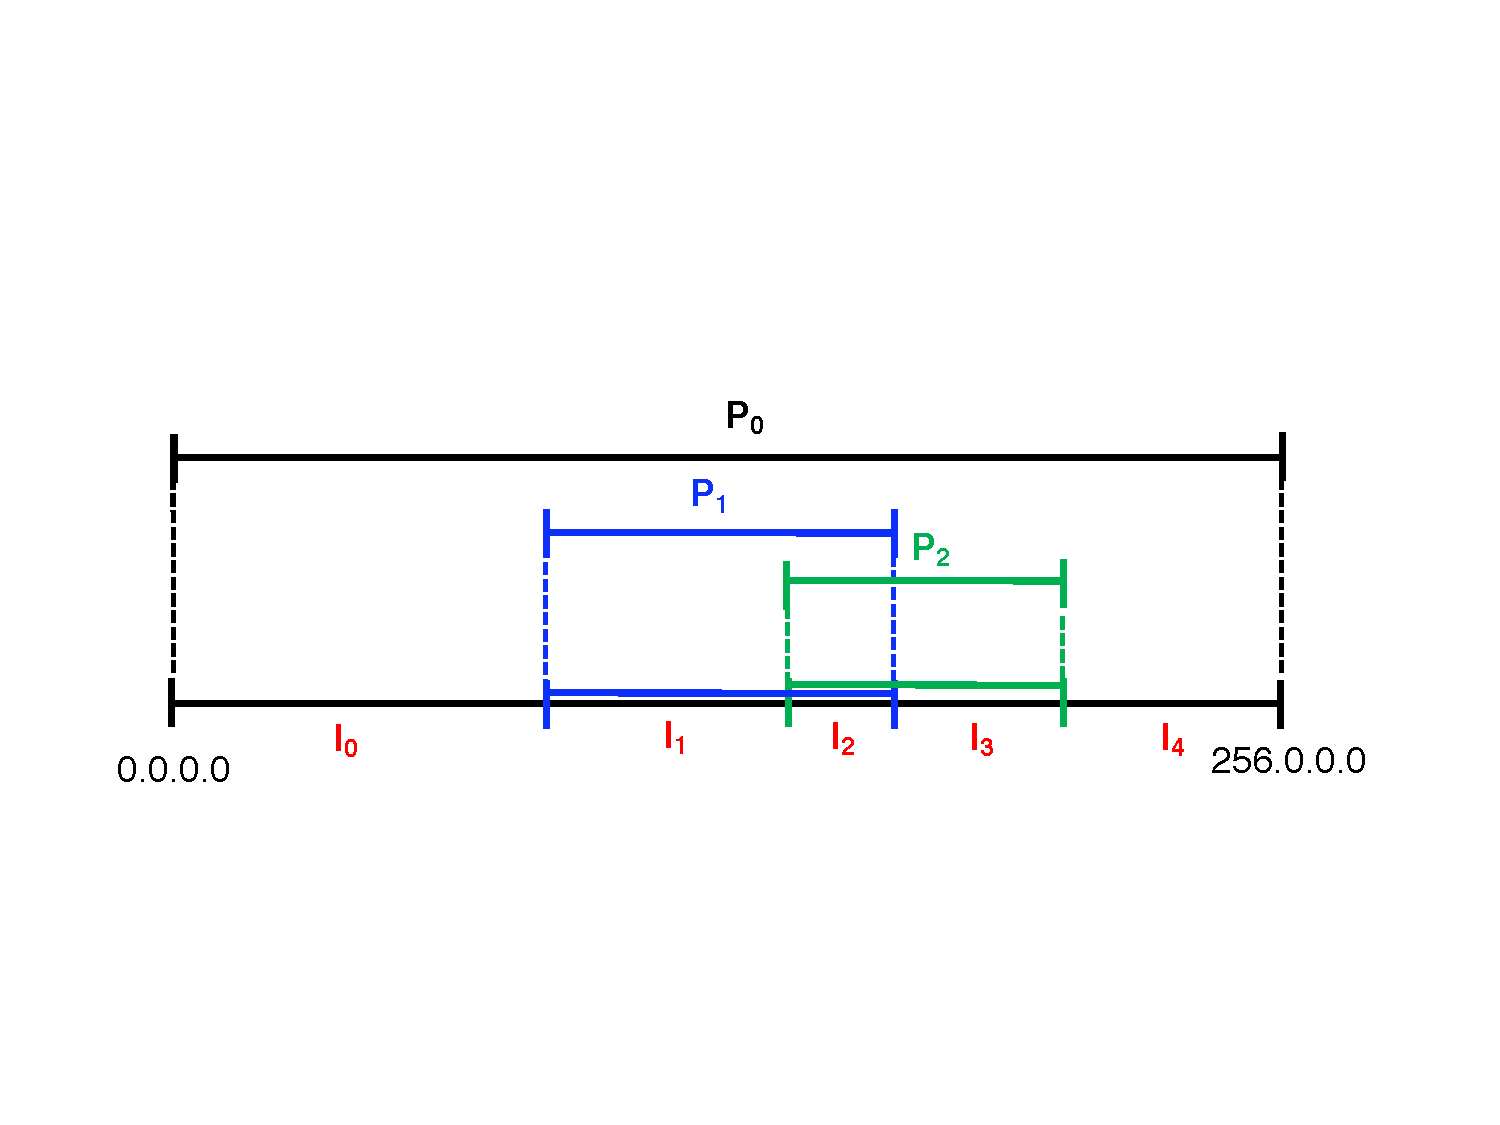
\includegraphics[width=3in]{fig/rangeopts3.pdf}
  \caption[]{Example of prefix encryption with PrefixMatch.\label{fig:rangeopts3}}
\end{figure}

We now explain how PrefixMatch works. To illustrate the protocol, we use IP addresses, but the scheme works with 
ports and other value domains too.



\mypara{Prefixes/ranges encryption} \pmatch{} takes as input a set of prefixes or ranges $P_1 = [s_1, e_1], \dots, P_n$, 
whose endpoints have size $\ptlen$ bits. \pmatch{} encrypts each prefix or range into a set of encrypted prefixes: these prefixes are $\plen$ bits long with a suffix of $\slen$. 

Consider all the endpoints $s_i$ and $e_i$ laid out on an axis in increasing order as in Fig.~\ref{fig:rangeopts3}.
Add on this axis the endpoints of $P_0$, the smallest and largest possible values, $0$ and $2^{\ptlen}-1$.
Consider all the intervals formed by each consecutive pair of such endpoints. 

For example, consider Fig.~\ref{fig:rangeopts3}.  There are two prefixes to encrypt: $P_1$ and $P_2$. PrefixMatch computes intervals $I_0, \dots, I_4$.

PrefixMatch now assigns an encrypted prefix to each interval. Note that each interval belongs to a set of prefixes. Let $\prefixes(I)$ denote the prefix of interval $I$. For example, $\prefixes(I_2) = \{P_0, P_1, P_2\}$. The encrypted prefix is simply a {\em random} number of size $\plen$. Each interval gets a different random value, except for the intervals that belong to the same prefixes. For example, in Fig.~\ref{fig:rangeopts3}, intervals $I_0$ and $I_4$ receive the same random number.

When an interval overlaps partially with another interval, it will have more than one encrypted prefix. For example, consider that $I_0$ was assigned a random number of $123:db8:85a3:::::$ and $I_1$ of $cdb:fa1:8$. The encryption of the prefix $P_1$ in Fig.~\ref{fig:rangeopts3} will be the pair ($123:db8:85a3:::::$, $cdb:fa1:8$).




Since the encryption is a random prefix, the encryption does not reveal the original prefix. Moreover, the fact that intervals pertaining to the same set of prefixes receive the same encrypted number hides where an encrypted value matches, as we discuss below. For example, for an IP address $v$ that does not match either $P_1$ or $P_2$, the cloud provider will not learn whether it matches to the left or right of $P_1$ and $P_2$ because $I_0$ and $I_4$ receive the same encryption. The only information it learns about $v$ is that $v$ does not match either $P_1$ or $P_2$. 

We now present the EncryptPrefixes procedure, which works the same for prefixes or ranges.



\begin{framed}
\ALGORITHM{EncryptPrefixes}{proc:enc_prefixes}{$P_1$, $\dots$, $P_n$, $\plen$, $\ptlen$, $\slen$}{
\item Let $s_i$ and $e_i$ be the endpoints of $P_i$. \comment{$P_i = [s_i, e_i]$}
	\item Assign $P_0 \gets [0, 2^{\ptlen}-1]$
	\item Sort all endpoints in increasing order
	\item  Construct intervals $I_0, \dots, I_m$ from each pair of consecutive endpoints. Multiple equal endpoints form a unit interval. For each interval $I_i$, compute $\prefixes(I_i)$, the list of prefixes $P_{1}, \dots, P_{m_i}$ that contain   $I_i$. 
	\item Assign a distinct random value of size $\plen$ to each of $\ov{I_0}, \dots, \ov{I_m}$  
	\item For all $i, j$ with $i<j$ if the prefixes containing $I_i$ and $I_j$ are the same, set $\ov{I_j} \gets \ov{I_i}$
	\item The encryption of $P_i$ is $\ov{P_i} = \{\ov{I_j}/\slen, I_j \in \prefixes(P_i) \}$. The encrypted prefixes are output sorted by value (as a means of randomization).
	\item Output $\ov{P_1}, \dots,\ \ov{P_n}$ and the {\em interval map} [$I_i \rightarrow \ov{I_i}$] 
}
\end{framed}

\mypara{Value encryption}
To encrypt a value $v$, PrefixMatch locates the one interval $I$ such that $v \in I$. $\ov{I}$ becomes the prefix of the encryption of $v$. This ensures that the encrypted $v$, $\ov{v}$, matches $\ov{I}/\slen$. The suffix of $v$ is chosen at random. The only requirement is that it satisfies the determinism property required in \todo{link}.
Hence, the suffix is chosen based on a pseudorandom function that $\prf^{\slen}$ seeded in a given seed  $\seed$.  



For example, if $v$ is 127.0.0.1, and the assigned prefix for the matched interval is $ads:241::::::/96$, a possible encryption given the ranges encrypted above is $Enc(v) = ads:241:3a3:90:ac:d:e:12$. Note that the ecryption does not retain any information about $v$ other than the interval it matches in. In particular, two values $v_1$ and $v_2$ that match the same interval, their order can be arbitrary. Thus, PrefixMatch does not reveal order.

\begin{framed}
\ALGORITHM{EncryptValue}{proc:enc_value}{$\seed$, $v$, $\slen$, interval map}{
\item Run binary search on interval map to locate the interval $I$ such that $v \in I$.
\item Lookup $\ov{I}$ in the interval map.
\item Output 
\begin{equation}
\Enc(v) = \ov{I} \Vert \prf_\seed^\slen(v)
\end{equation}
}
\end{framed}


%\begin{figure}
%  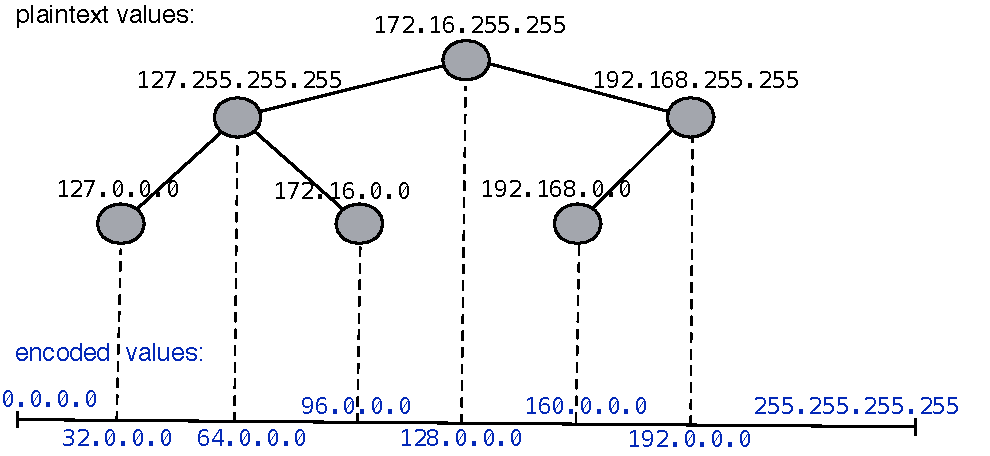
\includegraphics[width=3.25in]{fig/tree}
%  \caption{\label{fig:tree} PrefixMatch tree. The values of nodes in the tree are the %unencrypted IP addresses, and the blue values on the horizontal axis are their encryptions. }
%\end{figure}

\mypara{Comparing encrypted values against rules}
Determining if an encrypted value matches an encrypted prefix is straightforward: the encryption preserves the prefix.
Hence, a regular packet classification can be run at the firewall with no modification. Comparing different encrypted values for order that match the same prefix is meaningless, and returns a random value.




\subsubsection{Security Guarantees}

\pmatch{} hides the endpoints of ranges or the prefixes encrypted with EncryptPrefixes and it does not reveal the values encrypted with EncryptValue. \pmatch{} reveals only matching information between values and prefixes to enable functionality at the cloud provider.  For every subset of prefixes out of $P_1, \dots, P_m$, the cloud provider learns if these overlap and whether an encrypted value $v$ matches them. In particular, the cloud provider does not learn the order of encrypted values $\Enc(v)$ or the order of the prefixes. Hence, PrefixMatch is significantly more secure than order-preserving encryption.

%
Since the encryption is seeded in a per-connection identifier, correlation attacks between different flows are not possible. 
In particular, even though EncryptValue is deterministic, the encryption of the same IP address in different flows will be different because the seed differs per flow.
\todo{the above sentence needs some context}

We formalize and prove the security guarantees of \pmatch{} in our extended paper. 

\subsubsection{Implementing PrefixMatch in the Gateway}
\label{sec:tree}

\todo{THIS  SUBSECTION IS WORK IN PROGRESS}


\todo{move the following few in the gateway} We seed $\prf$ in $q$, a function of both the key and hash of the tuple being encrypted ($q = \prf_k(\text{(u, v)})$). Note that, in the system setup with two gateways, the gateways generate the same encryption because they share $k$. Let $N$ be $2^{w-m}$, where the value is $w$-bit and the prefix is $m$-bit. The encryption of $v$ is

The scheme supports NATs -- which require that every time a value for the same connection is encrypted, it returns the same value. It generates a random encryption using a deterministic function. 

When encrypting IP addresses, we do not want two different IP addresses to map to the same encryption (which would break the NAT). Fortunately, the probability that two IP addresses get assigned to the same encryption is negligibly low for IPv6.  The reason is that each interval of prefixes is large because we distributed the endpoints evenly and because there is a small number of such endpoints in a realistic setting (e.g., a firewall has less than 100,000 rules). Suppose we have $n$ distinct rules, $m$ flows and a $w$-bit space, with the assumption of uniformly distributed flows, the probability of getting collision is approximately 

\begin{equation}
1 - e^\frac{-m^2 (2n+1)}{2^{w+1}}
\end{equation}

\todo{discuss how the gateway gives the seed -- is the choice of seed outside of the prefixmatch alg or inside?}
\todo{discuss security of ports clearly}

Therefore, if $w=128$ (which is the case when we use IPv6), the probability is negligible in a normal setting. When encrypting ports, it is possible to get collisions since the port field is only 16-bit. However, this will not cause problem as long as the IP address does not collide, because NATs (and other middleboxes that require injectivity) considers both IP addresses and ports.

\todo{make clear that it is seeded in this so IPs do not collide}


\todo{need to discuss how the firewall puts prefix match in the prefix form, and adds /*}

\todo{remark for perfect security and tradeoff with work at the gateway}
\todo{does each rule become multiple rules?? explain who FW does with this, explain how many there are, need eval of this}
\todo{then in func you also need to clarfiy that it becomes more than one; this will leak about the prefixes what intersections they have!! even without fields matching}
\todo{and what does the firewall do?}


\todo{ I wonder how much of this section actually needs to move to the gateway section}

\todo{ need to discuss how the gateway chooses k for the encryptvalue -- the seed}

\noindent \textbf{Updating ranges.}
Adding a new range or removing an existing range would affect the intervals it covers. Therefore, in the worst case $O(N)$ rules needs to be updated. 

\todo{ and it has to be clear that to encrypt firewall rules at the gateway using the Prefix match, you need to go through each part of the rule and encrypt that; 
The gateway will use an instance of PrefixMatch for every field, destination IP, etc.
}
\todo{and need to discuss the prefix part}

\todo{need to discuss the fact that they blowup here}


The gateway stores the intervals and the mapping from intervals to prefixes for each field of the rules, and it maintains no state per IP address encrypted or per connection.

The gateway can use the following functions. EncryptRules encrypts the initial rules. EncryptTuple encrypts packet header fields which are represented as a tuple; it requires identifying the interval $I$ for each field. We can compute $I$ efficiently in logarithmic time by doing a binary search. 




% We now describe the procedure for AddRange which adds an interval (deleting an interval is similar). These procedures modify the state at the gateway. To add a range [$s$, $e$], the gateway inserts these values in the tree. If the tree needs to be rebalanced, for each endpoint that changed location in the tree, the gateway records the old and new encrypted value based on the tree in a list $L$. Note that  the number of endpoints that change encryption is $O(\log n)$ amortized worst-case. The gateway then computes the encryption of $s$ and $e$ based on their location in the tree. It sends to SP $\enc(s)$ and $\enc(e)$ along with $L$. 

%Besides the interval added or deleted, a small number
%of other intervals may be moved -- at worst, $O(\log n)$. 
%For these, the algorithm returns the old and new encryption of the interval. 

%
%\begin{framed}
%\begin{algorithmic}[1]
%
%\Procedure{AddRange}{$[s, e]$}
%  \State Insert $s$ and $e$ into the scapegoat tree. If $s=e$, insert the value only once.
%  %	
%  \State Initialize $L$ to be the empty list.
%  \If{tree needs to be rebalanced}
%  	\State Record which nodes change position in the tree during rebalancing, together with 
%	their old and new encryptions. Namely, record	\[L = \{ \en_1 \leftarrow \en^*_1, \dots, \en_m \rightarrow \en^*_m\},\] where $m$ is the number of nodes who changed position in the tree, and $\en_i$ and $\en^*_i$ are the old and new encryption of the $i$-th node that changed position. 
%  \EndIf
%  \State Compute  $\enc(s)$ and $\enc(e)$, the encryptions of $s$ and $e$, as in EncryptRanges.
%   \State \Return{$[\enc(s), \enc(e)], L$}
%\EndProcedure
%
%\end{algorithmic}
%\end{framed}

%  \State Determing the smallest and the largest encryption in the values $[\enc(s), \enc(e)]$ and $L$, and call this $\dirtyrange$.



\subsubsection{Rule Updates at the Cloud}
\label{sec:updates}
At the cloud, PrefixMatch poses two additional challenges to updating rules, both stemming from the fact that a rule update can also change encrypted values within packets.
The first challenge is middlebox state. Consider a NAT with a translation table containing ports and IP addresses for active connections
Adding or removing a rule will modify these values in the PrefixMatch tree, and thus to continue correct processing the NAT state must be updated.
The second challenge is a race condition: when the middlebox adopts a new ruleset while packets encrypted under the old tree are still flowing, these packets will be misclassified as their encryption values are inconsistent with the ruleset being applied. 
The same problem occurs if packets encrypted under the new tree arrive before the new ruleset.

To avoid these problems the gateway and cloud provider do the following. 
When the gateway updates the PrefixMatch tree, it announces to the cloud provider of the pending update, and the middleboxes ship their current state to the gateway to receive the new encryption values.
The gateway then sends a signal to the cloud provider that it is about to `swap in' the new map. 
The cloud provider buffers traffic for a few hundred milliseconds after this signal to allow all old traffic to complete processing at the cloud; it signals to all middleboxes to `swap in' the new rules and state; and finally it releases the new traffic.
Note that all changes to middleboxes are in the {\it control plane} of the middlebox, and require no modifications to the algorithms and operations performed in per-packet processing. 

